\begin{figure}[h]
	\centering
	
\includegraphics[scale=2.5]{03_Bedienungsanleitung/img/Logo_HFTl_App.png}
	\label{img:grafik-dummy}
\end{figure}

\begin{center}
	{\huge Benutzerhandbuch}
\end{center}

\begin{center}
	{\huge -  HfTL-APP  -}
\end{center}



\newpage
\subsection{Benutzerhandbuch}
\subsubsection{Funktionsumfang}
In diesem Dokument wird die Benutzerfunktionen von der HfTL-APP für
Android-Geräte beschrieben. Es dient als Benutzerhandbuch für die
unterschiedlichen Funktionen der Anwendung und soll Ihnen beim
Ausführen von häufigen Aktionen innerhalb der Anwendung Hilfe bieten.
Die Installation und Konfiguration von der HfTL-APP wird in einem
separaten Dokument behandelt.

Die HfTL-APP ist eine mobile Informationslösung für Android Geräte. Die App kann kostenlos über das Rechenzentrum der Hochschule für Kommunikation-Leipzig bezogen werden.

Die HfTL-APP bietet folgende Funktionen:

\begin{itemize}
\item Abfrage der News von der HfTL-Homepage
\item Abfrage der Noten aus QIS/HIS nach erfolgreicher Anmeldung an dem betreffenden System
\item Abfrage des zu einem Studenten passenden Stundenplans
\end{itemize}

HINWEIS: In diesem Dokument wird vorausgesetzt, dass die HfTL-APP bereits installiert ist.
\begin{figure}[h]
	\centering
	\includegraphics[scale=0.5]{03_Bedienungsanleitung/img/appstore.jpg}
	%\caption{eine Grafik ohne Sinn und Verstand}
	\label{img:grafik-dummy}
\end{figure}

\newpage

\subsubsection{Startbildschirm}


\begin{figure}[h]
	\centering
	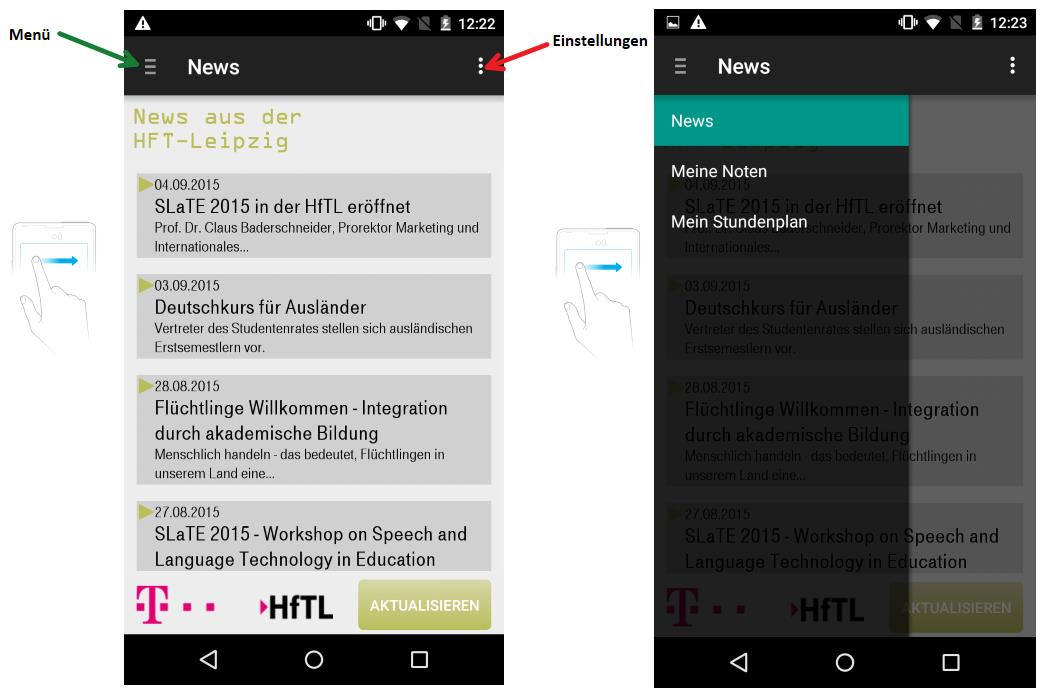
\includegraphics[scale=0.8]{03_Bedienungsanleitung/img/start2.jpg}
	%\caption{eine Grafik ohne Sinn und Verstand}
	\label{img:grafik-dummy}
\end{figure}

%\begin{wrapfigure}{r}{0.5\textwidth}
  %\begin{center}
   % 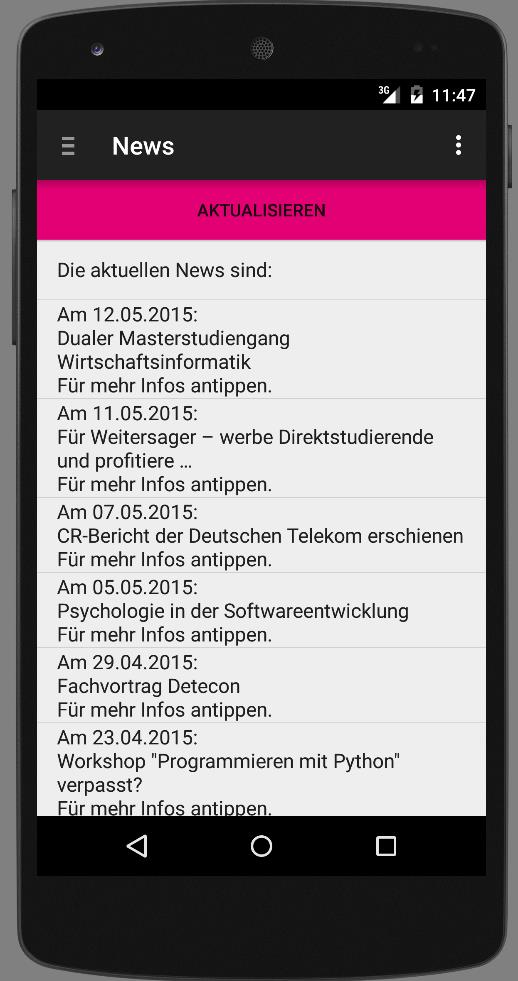
\includegraphics[width=0.5\textwidth]{03_Bedienungsanleitung/img/start.jpg}
  %\end{center}
  %\caption{HFTL-APP©gemeinfrei}
 % \label{reaper}
%\end{wrapfigure}

Nach Starten der APP erscheint zunächst die News-Seite. Die News werden bei bestehender Internetverbindung automatisch aktualisiert. Mit klicken auf den Aktualisierungsbutton kann eine manuelle Aktualisierung durch den Nutzer angestoßen werden.

Über den Menü-Button gelangt der Nutzer in das Programm-Menü. Über den Einstellungs-Button gelangt man in das Einstellungs-Menü.
Mit Auswählen der einzelnen News gelangt man in deren Detailansicht.

\newpage
\subsubsection{Newsansicht}
\begin{figure}[h]
	\centering
	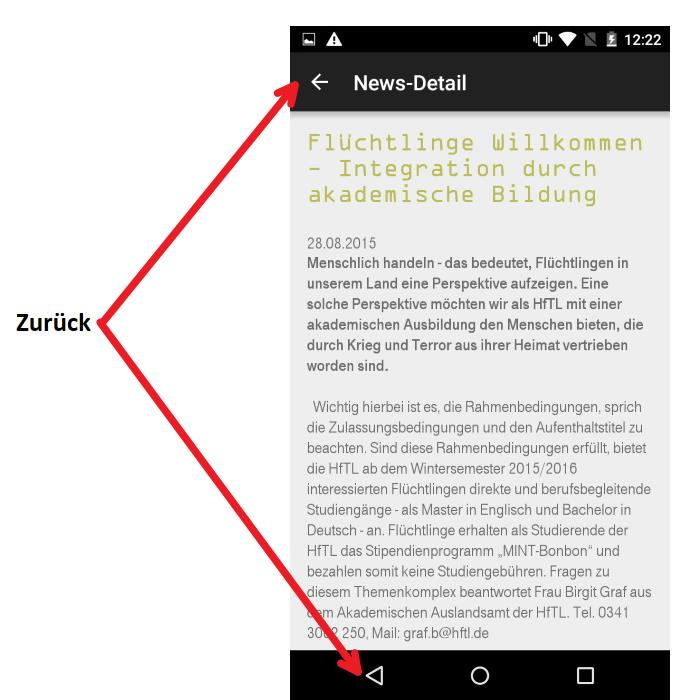
\includegraphics[scale=0.8]{03_Bedienungsanleitung/img/news.jpg}
	%\caption{eine Grafik ohne Sinn und Verstand}
	\label{img:grafik-dummy}
\end{figure}

Mit den Zurück-Buttons gelangt man in die vorherige Ansicht.

\newpage
\subsubsection{Noten}

Um die Noten abzurufen geht man zunächst in den Einstellungskontext. Dort kann der Nutzer und das jeweilige Passwort eingegeben werden.
\\
\\
Mit einem Klick auf Benutzername bzw. Passwort öffnet sich ein neuer Kontext welcher zum eingeben des Benutzernamens bzw. Passwortes auffordert.
\\
\\
Die Eingabe wird mit "'OK"' gespeichert und mit "'Abbrechen"' verworfen. Bei beiden Aktionen schließt sich der Kontext.

\begin{figure}[htb]
    \centering
    \begin{minipage}{0.45\linewidth}
        \centering
        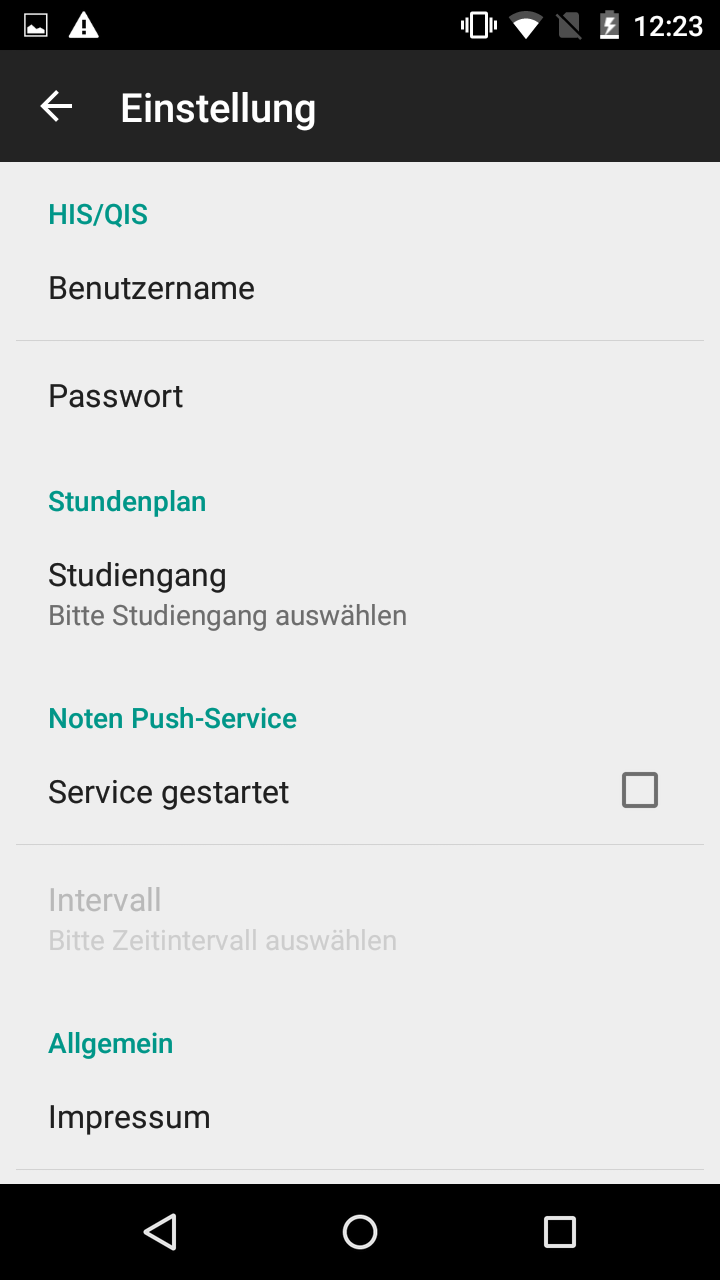
\includegraphics[scale=0.5]{03_Bedienungsanleitung/img/einstellungen.png}
        %\caption{Beispielbild b}
    \end{minipage}
    %\hfill
    \begin{minipage}{0.45\linewidth}
        \centering
        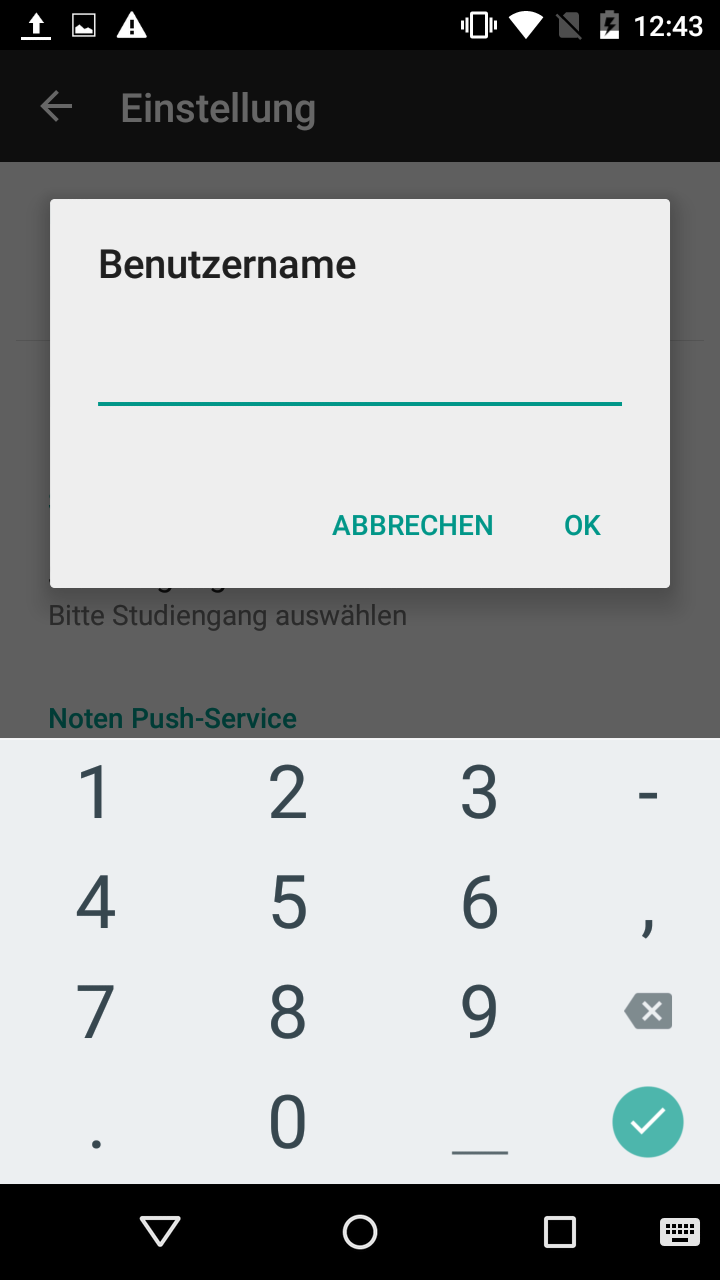
\includegraphics[scale=0.5]{03_Bedienungsanleitung/img/account.png}
        %\caption{Beispielbild b}
    \end{minipage}
\end{figure}

\newpage

Nach erfolgreichem Eintragen des Benutzeraccounts und verlassen der Einstellungen kann über den Menü-Button der Punkt "Noten" ausgewählt werden. Hier werden die aktuellen Noten aus QIS/HIS geladen und angezeigt. Sollte es beim Anmelden an QIS/HIS zu einem Fehler kommen, erscheint eine Fehlermeldung und die vorher vorgenommenen Einstellungen sollten noch einmal kontrolliert werden. 

\begin{figure}[h]
	\centering
	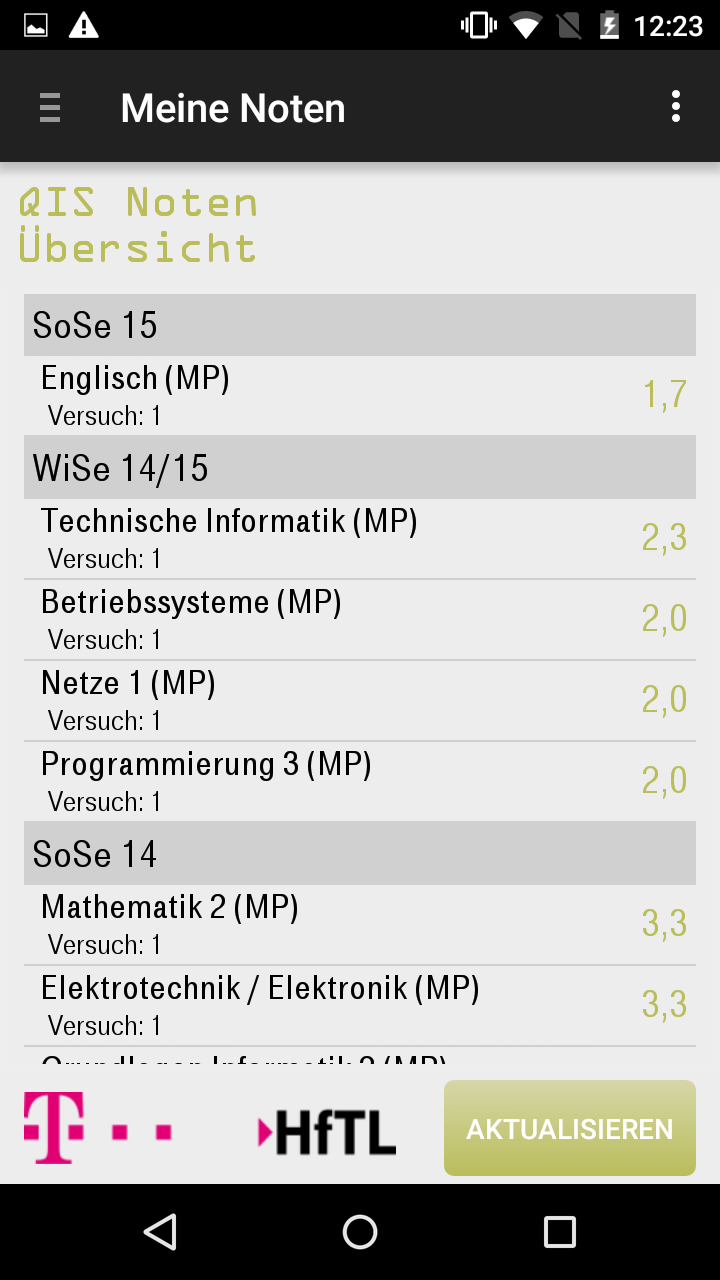
\includegraphics[scale=0.6]{03_Bedienungsanleitung/img/noten.png}
	%\caption{eine Grafik ohne Sinn und Verstand}
	\label{img:grafik-dummy}
\end{figure}

\newpage

\subsubsection{Stundenplan}

Den Stundenplan erreicht man über das Menü. Hat man in den Einstellungen vorher seinen Studiengang und das Matrikeljahr angegeben, erscheint dazu passende Stundenplan.

\begin{figure}[h]
	\centering
	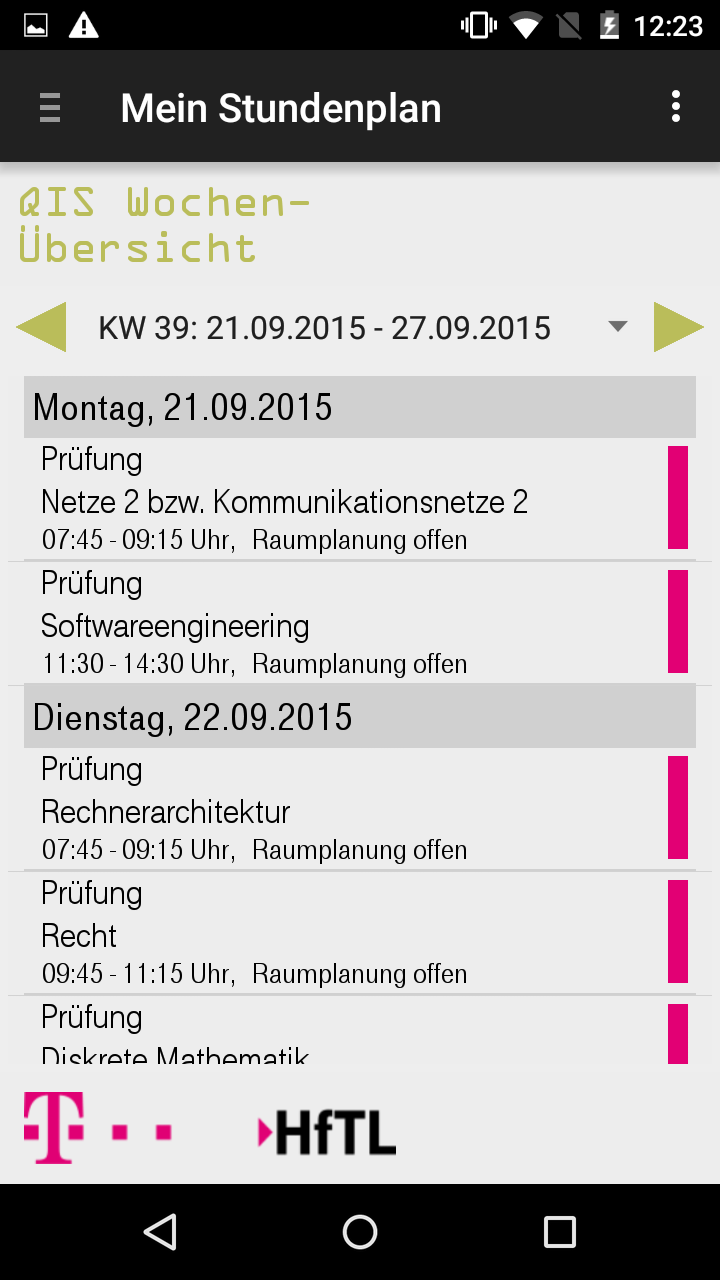
\includegraphics[scale=0.6]{03_Bedienungsanleitung/img/stundenplan.png}
	%\caption{eine Grafik ohne Sinn und Verstand}
	\label{img:grafik-dummy}
\end{figure}

